\chapter{GRIPPER DESIGN}
\graphicspath{{./}{pictures/}{inventor/}}
\section{Requirements of objective}
Picking asparagus with a robotic arm requires a carefully coordinated process that prioritises gentle handling and consistent performance while minimising damage to the plant. The gripper must interface reliably with slender, fragile spears, accommodating natural variability in diameter, length, and orientation. To enable this, the system first detects the presence of asparagus plants in the field and accurately estimates the position, pose, and size of individual spears.

Perception can be achieved using cameras, LiDAR, or a sensor fusion approach that balances accuracy, robustness, and cost. Visual or depth sensing provides the measurements necessary to localise each spear within the robot’s workspace and to categorise targets according to maturity and suitability for harvesting. These classifications inform grasp strategy—such as contact location, applied force, and approach vector—so that the gripper can secure the spear without bruising, bending, or uprooting adjacent growth. This sensing-to-action pipeline underpins the design requirements for the gripper, ensuring that mechanical, sensing, and control choices collectively support precise, repeatable, and low-damage harvesting.




\section{Finger design}
For a finger design to pick and chop the stem of asparagus, I have set up a design based on
two fingers which will hold the asparagus stem down by a mg995 servo motor adjunct with a
and a blade holder underneath the finger also driven by another servo mg995. The whole
design is worked on inventor 2025 as it could be seen below


\begin{figure}[H]
    \centering
    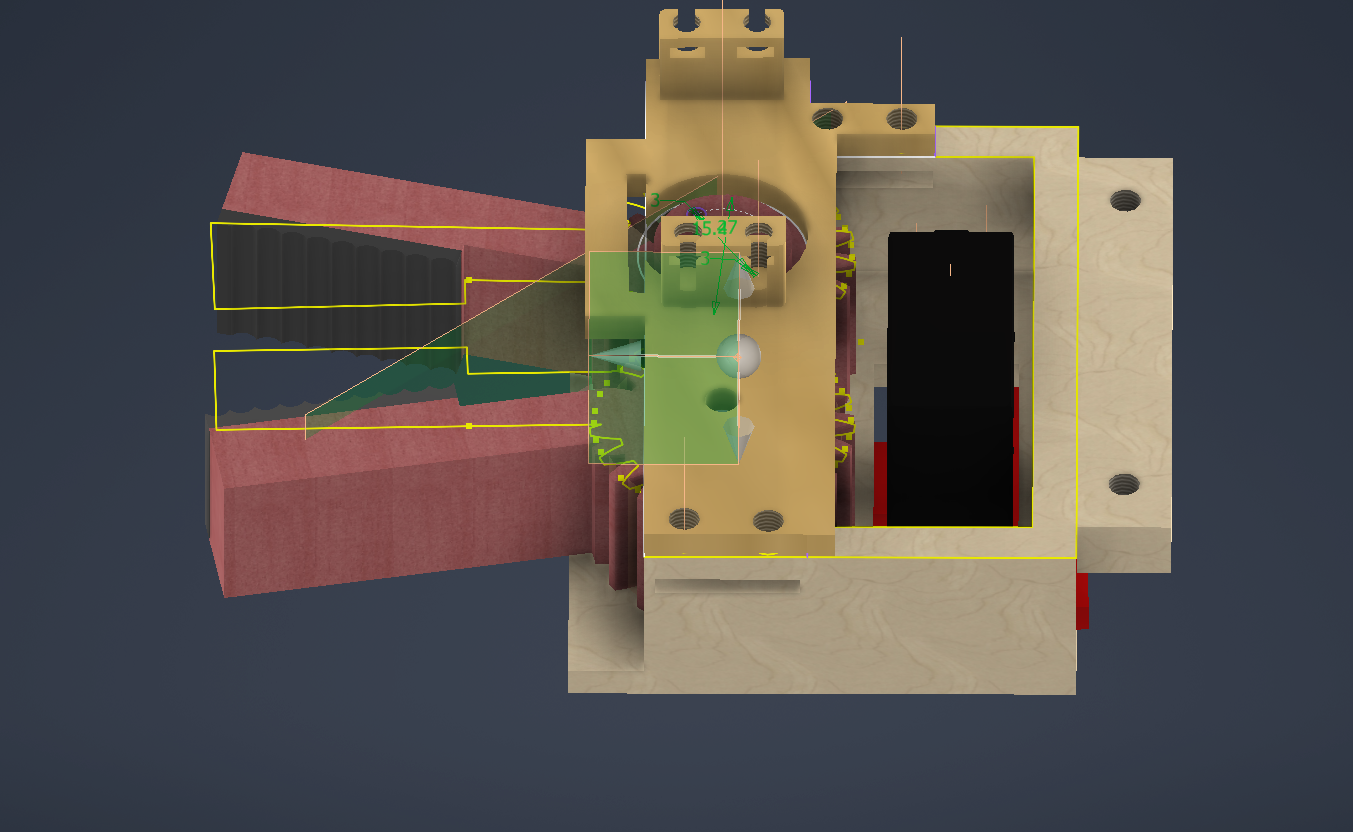
\includegraphics[width=0.9\textwidth]{finger_design_inventor.png}
    \caption{Finger design developed in Inventor 2025 showing kinematics and packaging.}
    \label{fig:finger_inventor}
    \end{figure}








The red component in Figure~\ref{fig:finger_inventor} denotes the finger module, which achieves a
form-closure grasp on the asparagus spear. The grasping strategy is intentionally conservative to
avoid bruising or buckling of the slender stem. To this end, the contact surfaces are equipped with
compliant, sponge-like pads that deform elastically, distributing pressure over a larger area and
attenuating transient load peaks during closure. The applied normal force is limited to a target
maximum of approximately 10\,N, which is adopted as a safe threshold for handling without damage
based on empirical observations from preliminary trials.

To verify that these constraints are satisfied across expected geometric and material variability, the
finger will be evaluated through a combination of quasi-static and dynamic analyses. The study will
include contact modelling of the pad–spear interface, estimation of required actuation torque under
frictional form closure, and time-domain simulations to quantify impact forces during grasp onset and
blade engagement. These results will inform controller tuning and pad material selection, ensuring the
design achieves reliable retention while preserving the integrity of the crop.



To quantify actuator demands, a time-domain dynamic analysis was performed to estimate the
resultant torque at the finger joint under a conservative handling load. Assuming a maximum
allowable contact force of approximately 10\,N at the fingertip, the corresponding joint torque
was computed over the grasping trajectory. The simulation was executed in Autodesk Inventor
2025 using 100 time steps to capture transient effects and peak values in Decinewton (dN). The resulting torque
profile is shown in Figure~\ref{fig:finger_torque}.
\begin{figure}[H]
    \centering
    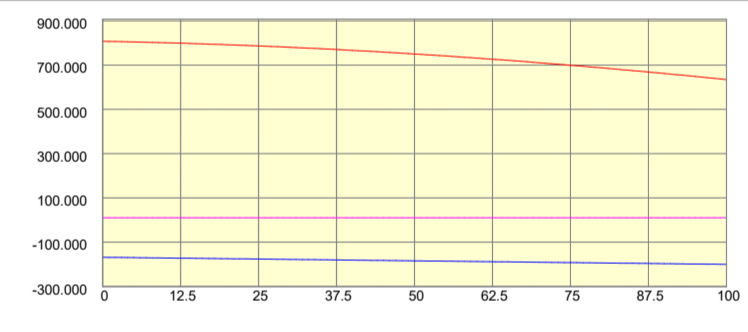
\includegraphics[width=0.75\textwidth]{fingerforceDynamics.png}
    \caption{Computed finger joint torque over the grasping trajectory (100-step dynamic analysis).}
    \label{fig:finger_torque}
    \end{figure}

    


\section{Electrical schematic and operation}


\begin{figure}[H]
    \centering
    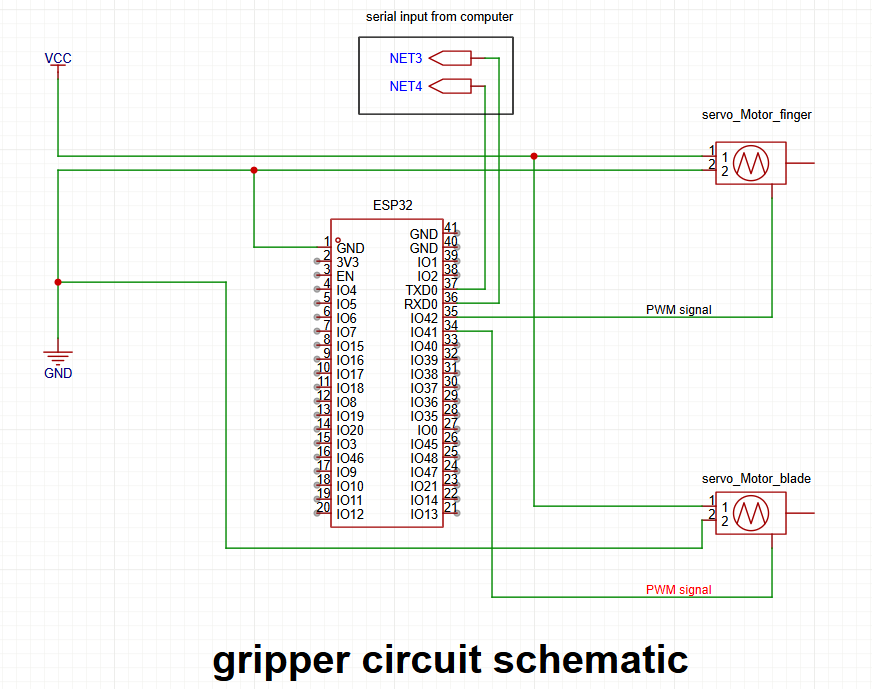
\includegraphics[width=0.9\textwidth]{gripperschamatics.png}
    \caption{Electrical schematic of the gripper controller based on ESP32.}
    \label{fig:gripper_schematic}
    \end{figure}

Figure~\ref{fig:gripper_schematic} presents the electrical schematic for the gripper subsystem. The
ESP32 serves as the central controller and receives high-level commands either via a wired serial
link from a host computer or through Bluetooth Serial communication. A real-time operating system
(RTOS) is employed to schedule the two principal tasks—finger actuation and cutting blade
actuation—so that each executes without blocking or degrading the performance of the other.

Pulse–width modulation (PWM) signals are generated directly by the ESP32 to command the servos.
The finger servo (MG992) is driven from pin IO42, while the blade servo is driven from pin IO41.
These assignments allow independent, deterministic control of grasping and cutting actions, with
timing guarantees provided by the RTOS tasks.

The gripper electronics are powered by a regulated 5\,V supply sized to accommodate concurrent
servo transients; the servo ground is tied to the ESP32 logic ground to ensure a common reference
for PWM signalling. Reference firmware and the associated GitHub repository link are provided
in the Appendix for reproducibility and implementation details.




\section{End-effector fabrication and assembly}

This section documents the physical realisation of the gripper and cutter. Printed parts were
fabricated with fine layers for contact surfaces and higher infill for load-bearing features, then
post-processed by drilling/reaming critical holes to final size. The figures below summarise key
subassemblies and the final integration.


\begin{table}[H]
    \centering
    \caption{Bill of materials for the prototype gripper and cutter.}
    \label{tab:gripper_bom}
    \resizebox{\textwidth}{!}{%
    \begin{tabular}{l c l l}
        \hline
        \textbf{Item} & \textbf{Qty.} & \textbf{Specification} & \textbf{Function} \\
        \hline
        ESP32 development board & 1 & Wi‑Fi/Bluetooth MCU & Central controller, PWM generation \\
        Servo motor (MG995) & 2 & Metal gear, high torque & Finger actuation; blade actuation \\
        Cutting blade & 1 & Utility/trapezoidal blade & Stem cutting element \\
        PLA filament & — & 1.75\,mm, standard grade & Structural parts: gripper and housing \\
        TPU filament & — & 1.75\,mm, shore 95A (approx.) & Compliant soft fingertip pads \\
        \hline
    \end{tabular}%
    }
    \end{table}

The ESP32 provides integrated wireless connectivity and sufficient timers for dual PWM outputs,
enabling deterministic control of both servos. MG995 units were selected for their readily available
torque capacity and robustness for prototyping. PLA is used for the primary structure due to its
dimensional stability and ease of printing, while TPU is employed at the fingertip interfaces to
introduce compliance that distributes contact pressure and mitigates damage to the asparagus spear.
The replaceable utility blade affords a sharp, low-mass cutting edge suitable for repeatable stems
severing during trials.



\begin{figure}[H]
    \centering
    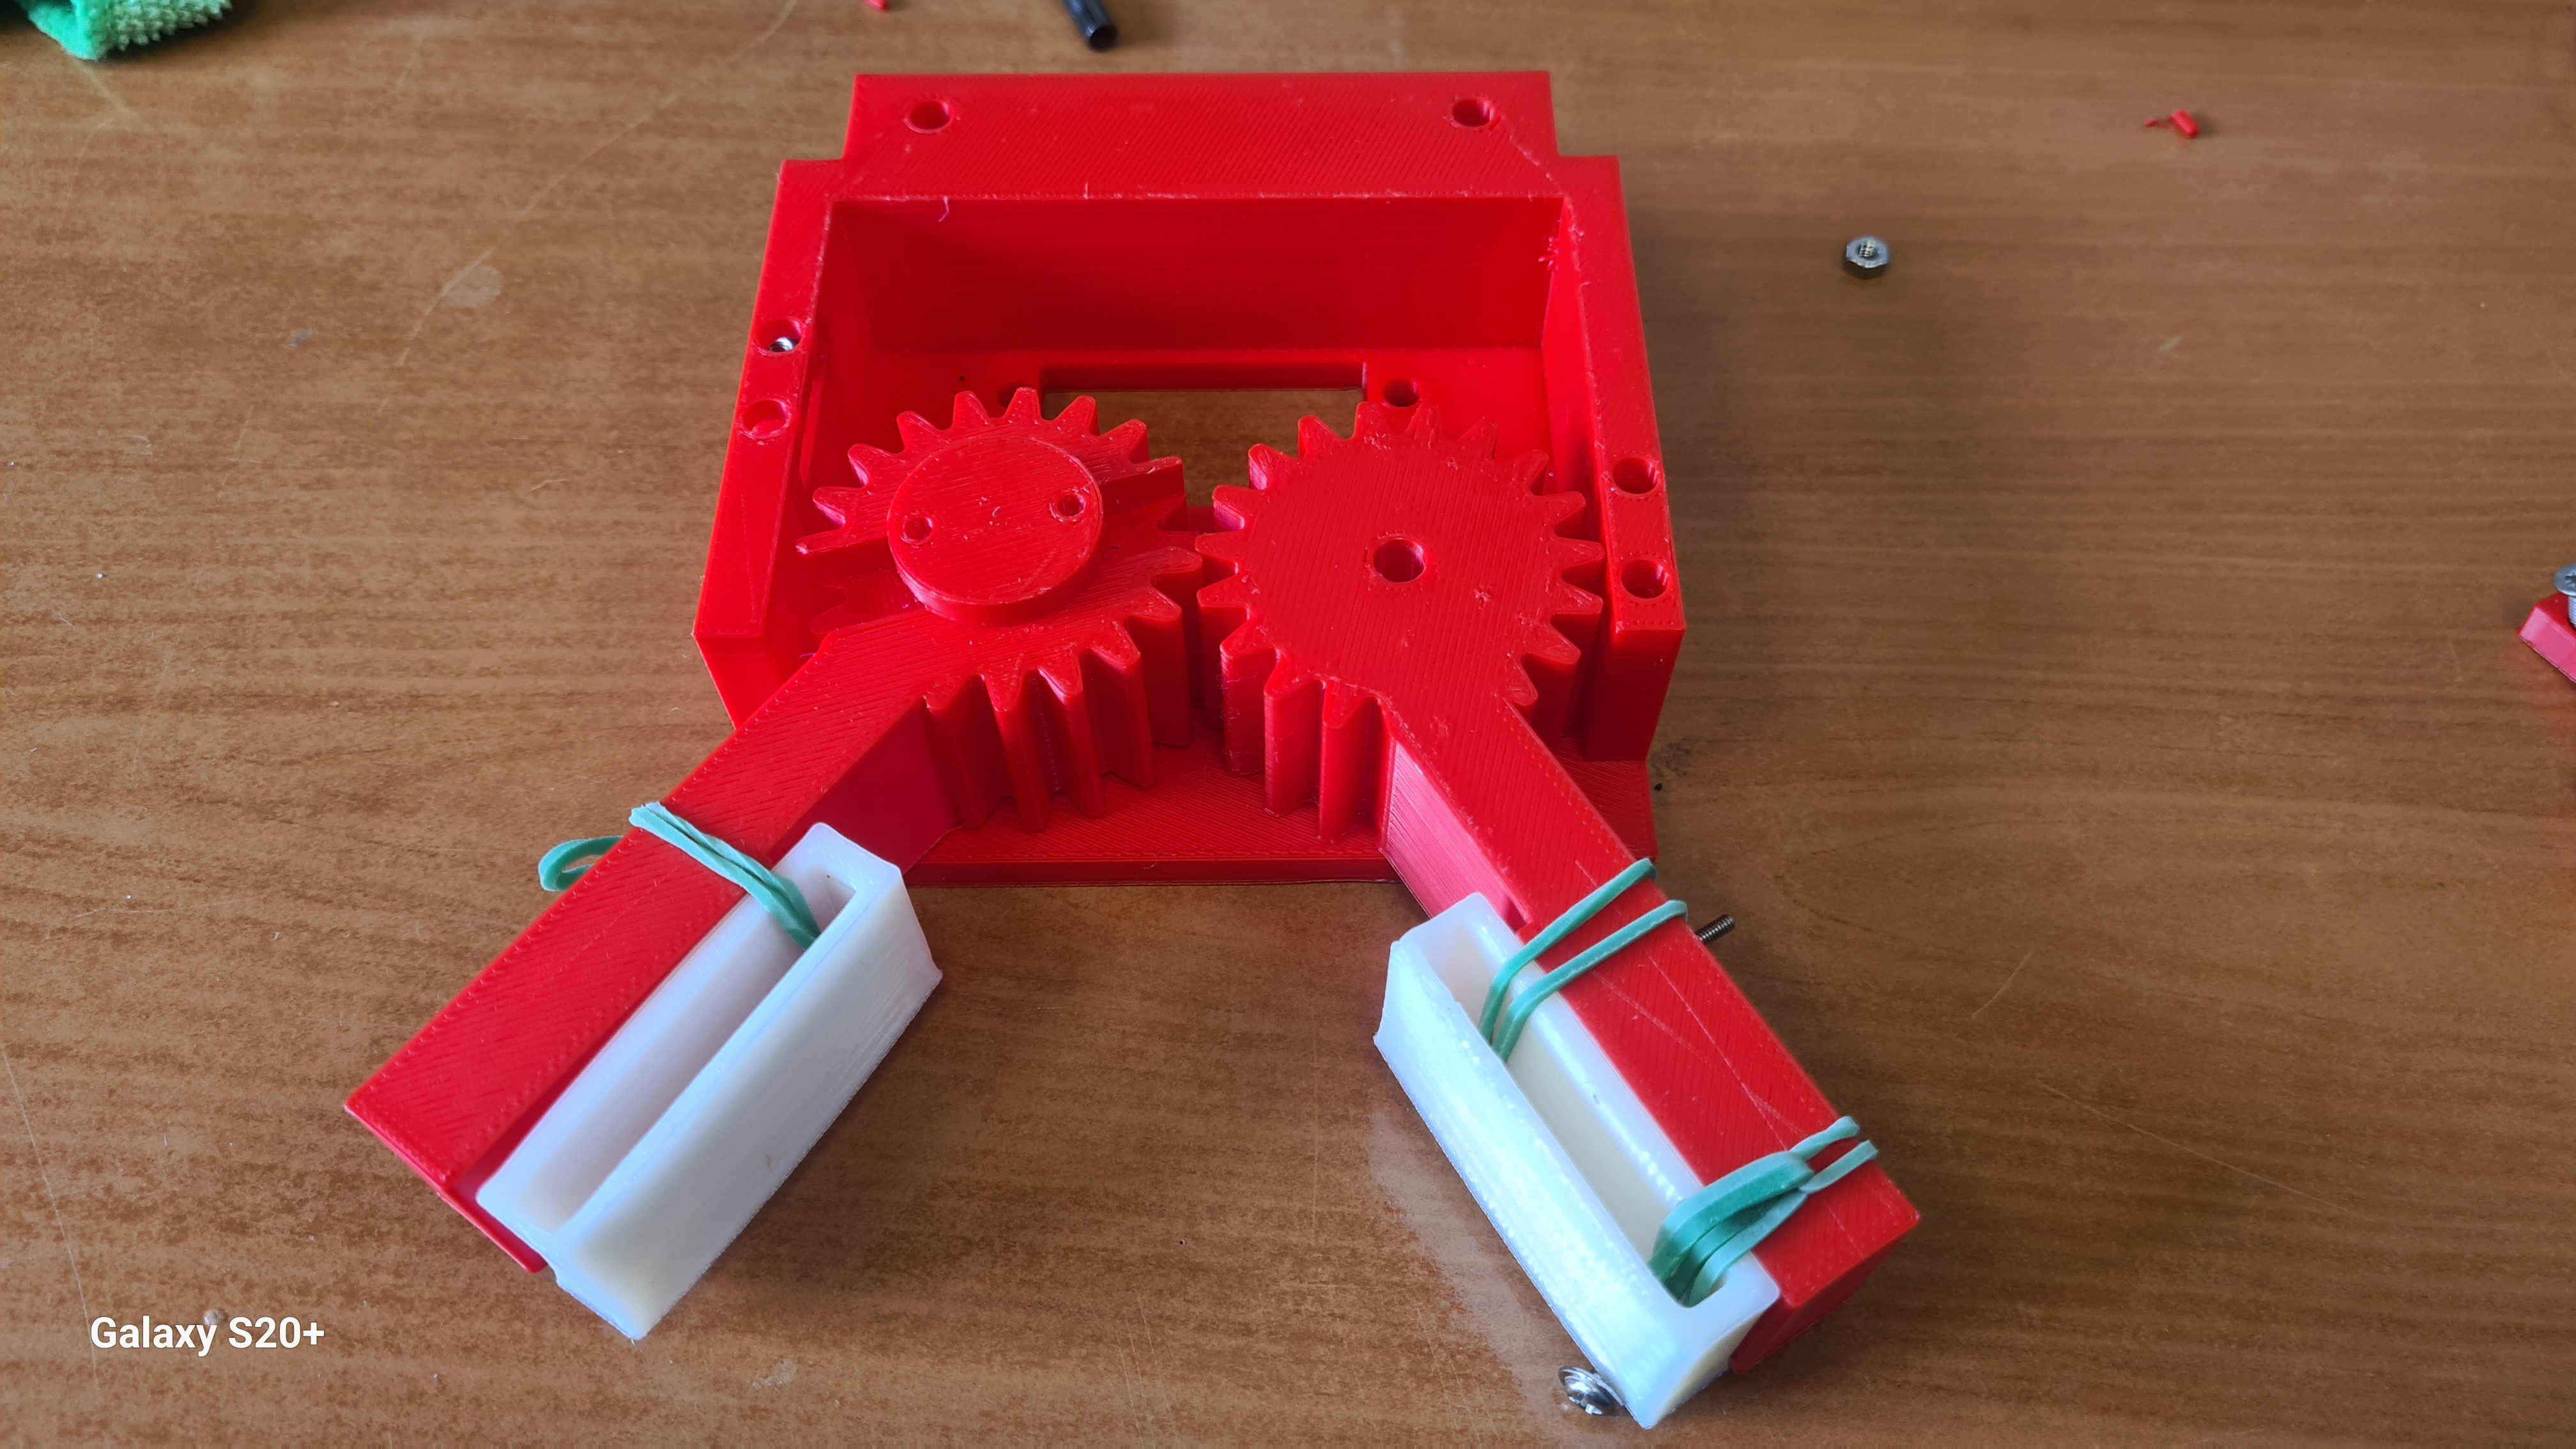
\includegraphics[width=0.9\textwidth]{fingerGear.jpg}
    \caption{Finger actuation gears illustrating the symmetric closing mechanism.}
    \label{fig:finger_gears}
    \end{figure}
    
    Figure~\ref{fig:finger_gears} depicts the printed spur-gear pair used to kinematically
    synchronise the two fingers. The arrangement enforces equal and opposite angular motion,
    yielding symmetric closing and reliable centring of the spear prior to cutting. Gear modules
    and tooth counts were selected to balance compact packaging with adequate torque capacity;
    backlash was minimised through post-processing of bores and the use of press-fit pins with
    lubrication applied after assembly. This configuration reduces differential slip at the contacts
    and improves repeatability of the grasping pose across cycles.
    

\begin{figure}[H]
\centering
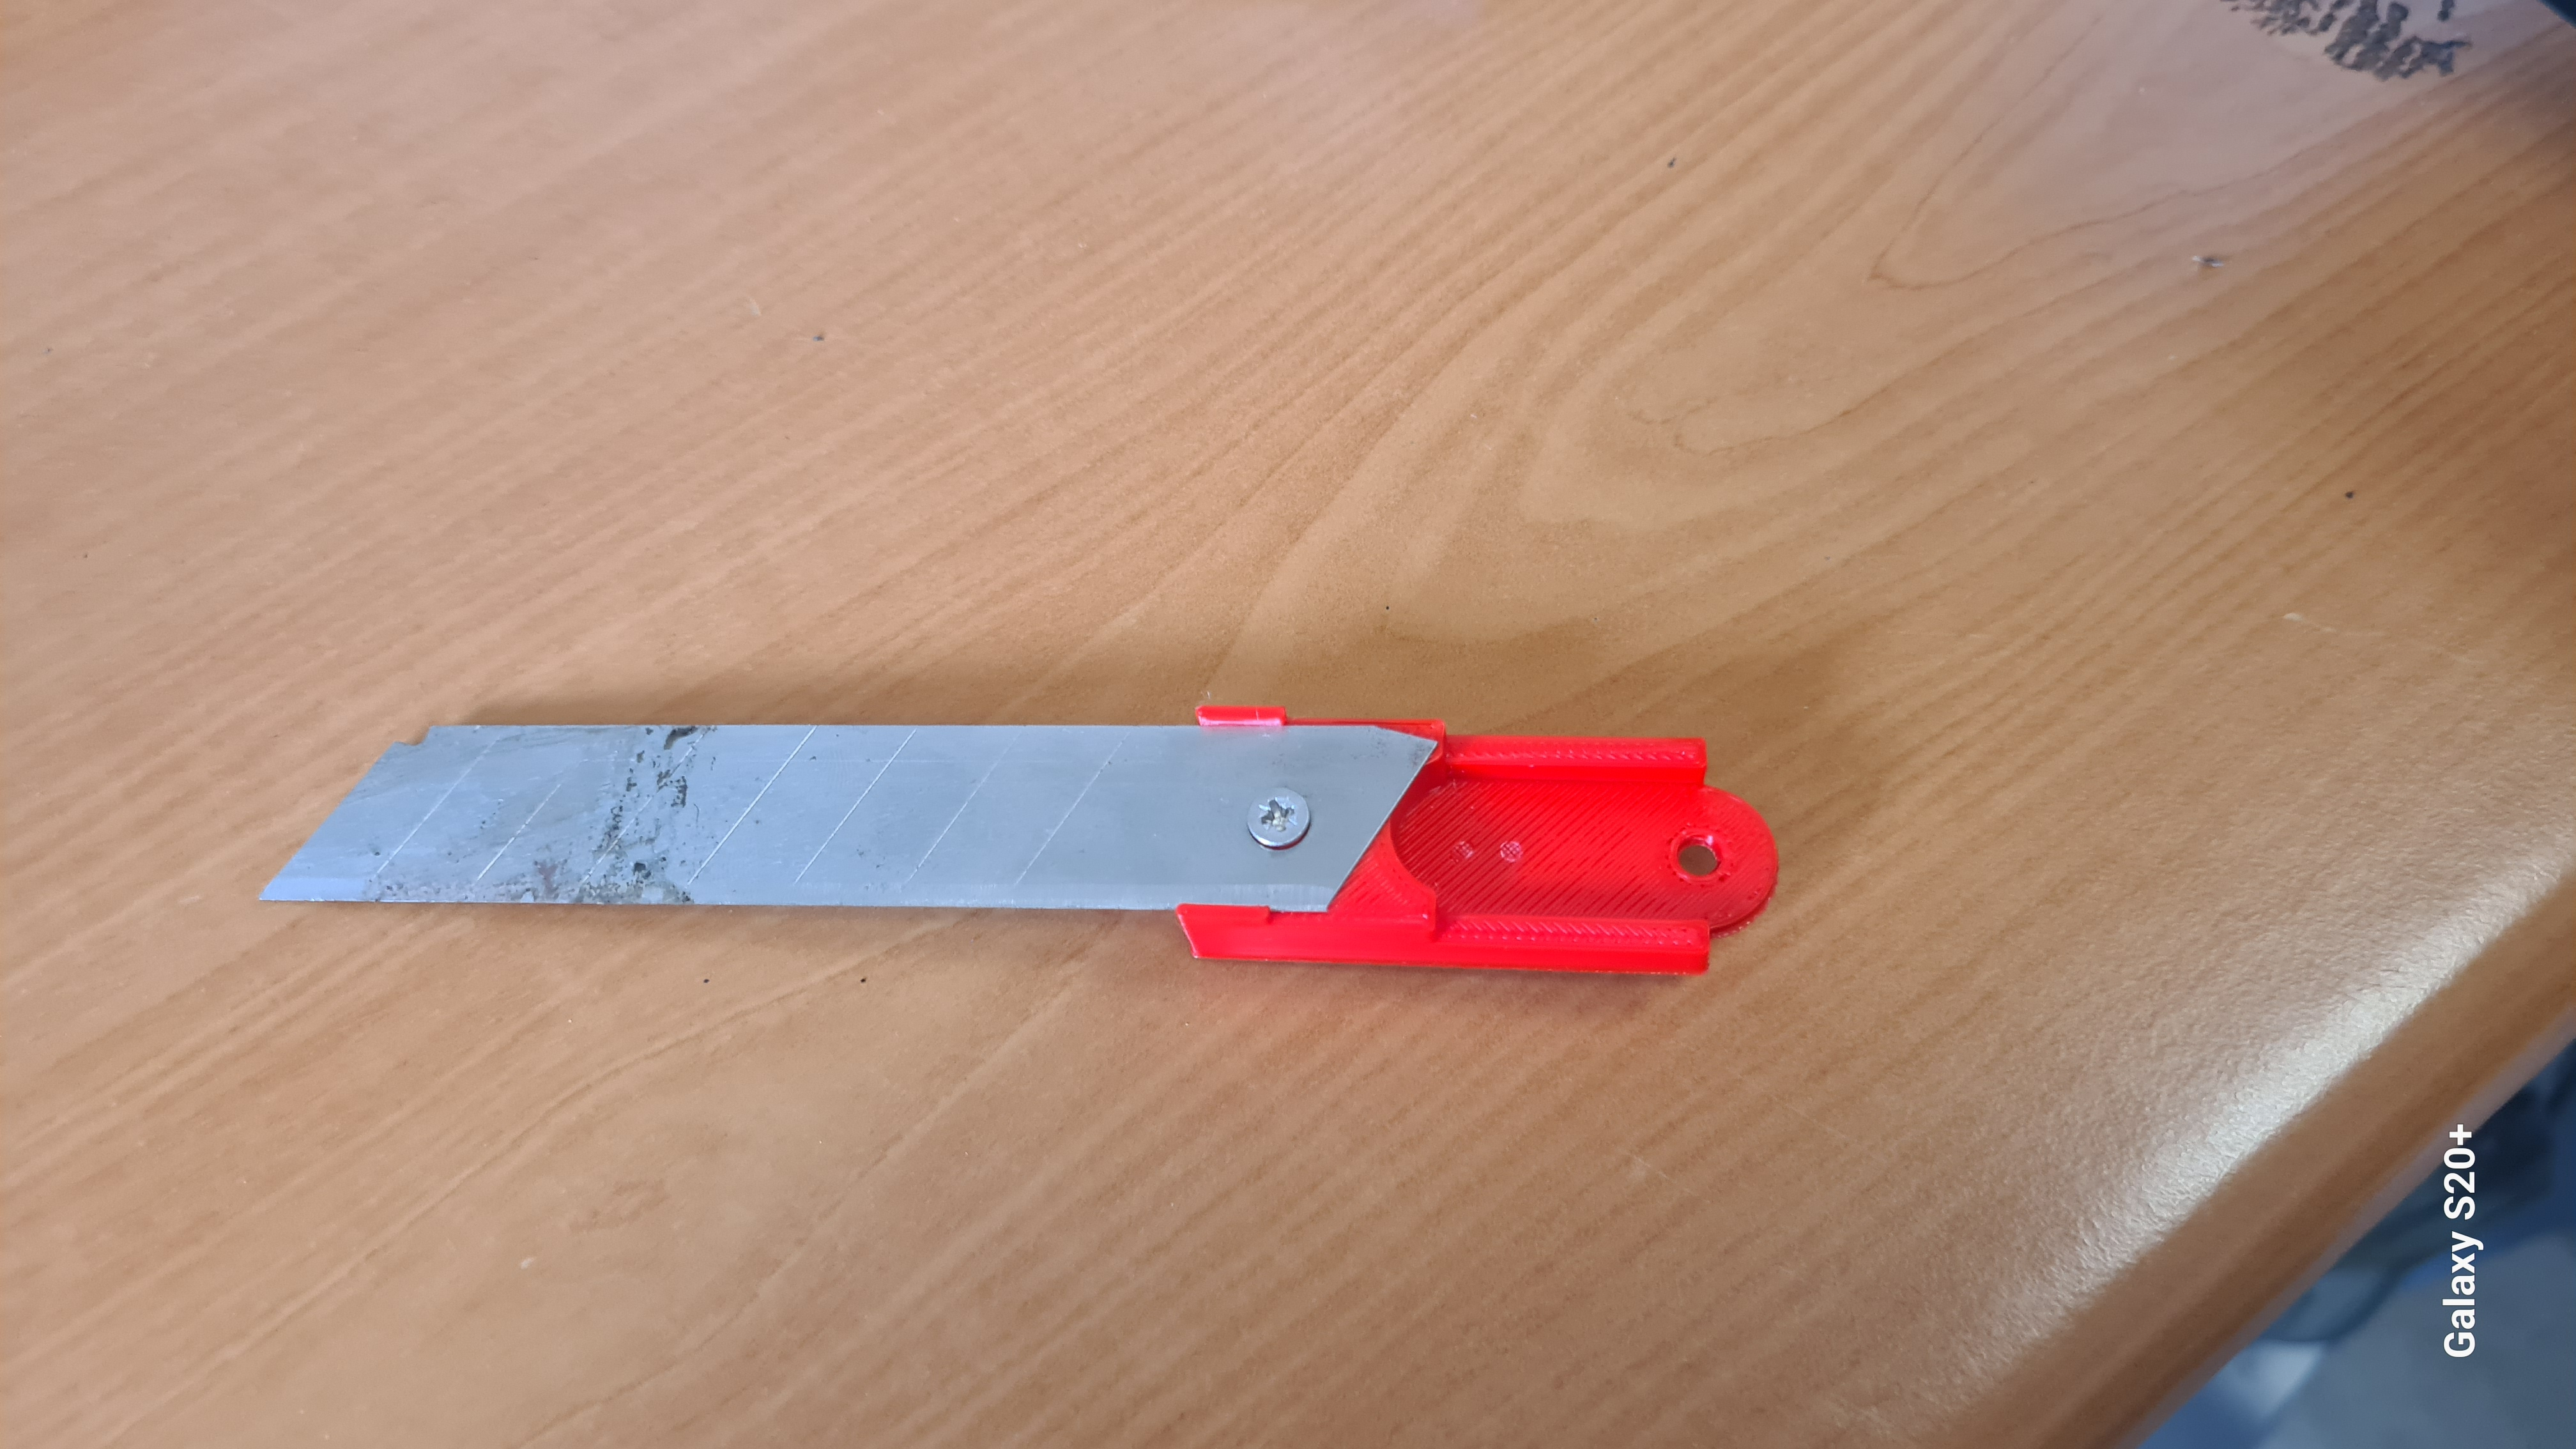
\includegraphics[width=0.75\textwidth]{Blade.jpg}
\caption{Blade prototype for asparagus stem cutting.}
\label{fig:blade}
\end{figure}

Figure~\ref{fig:blade} shows the replaceable utility blade secured within a low-mass carrier used
for early trials. A standard trapezoidal blade was selected for availability, edge sharpness, and
cost. The carrier constrains the blade in-plane while allowing straightforward replacement,
facilitating iterative testing of attack angle and exposure. Preliminary trials focused on edge
durability, required stroke force, and the effect of blade orientation on cut quality.

\begin{figure}[H]
\centering
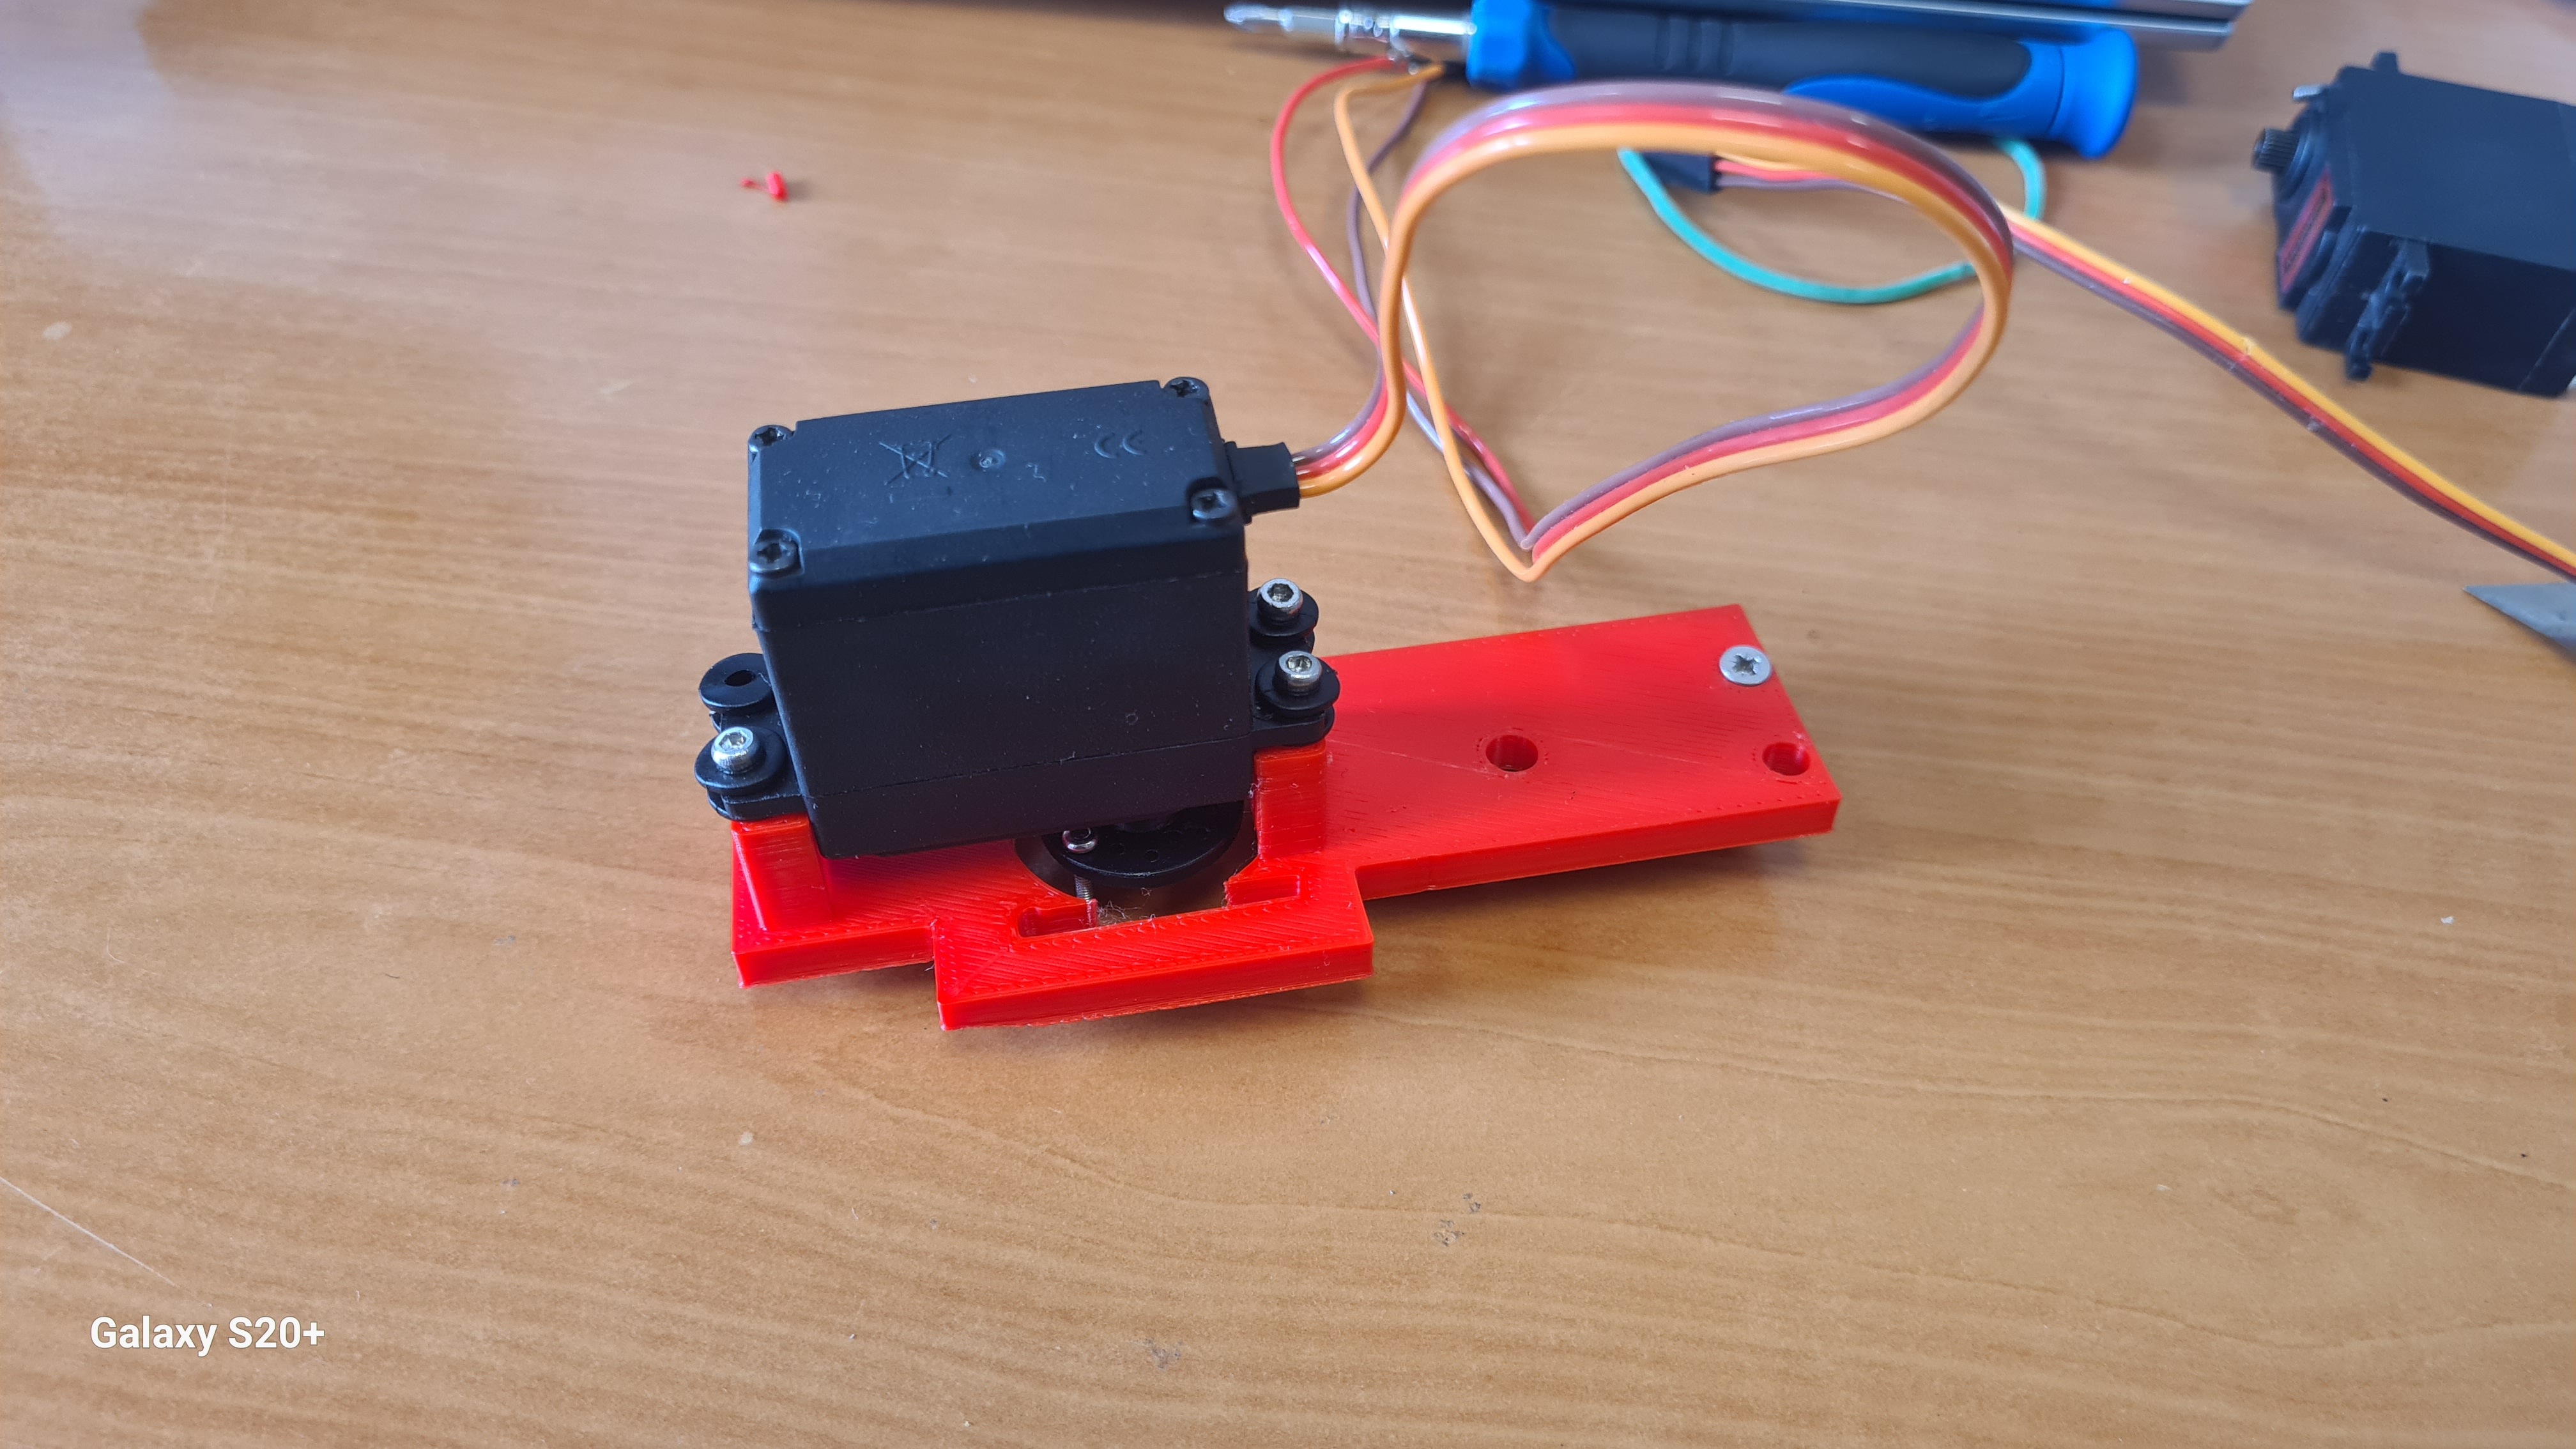
\includegraphics[width=0.85\textwidth]{bladeDriverandMount.jpg}
\caption{Blade driver and mounting arrangement with servo actuation.}
\label{fig:blade_driver_mount}
\end{figure}

Figure~\ref{fig:blade_driver_mount} illustrates the servo-driven blade mount. The blade carrier is
coupled to a high-torque servo through a rigid hub and supported by bushings to constrain
out-of-plane motion. The mount geometry establishes a repeatable attack angle relative to the
stem and limits lateral compliance that could degrade cut quality. Cable routing and fastener
access were considered to enable maintenance and rapid blade exchange during field operation.

\begin{figure}[H]
\centering
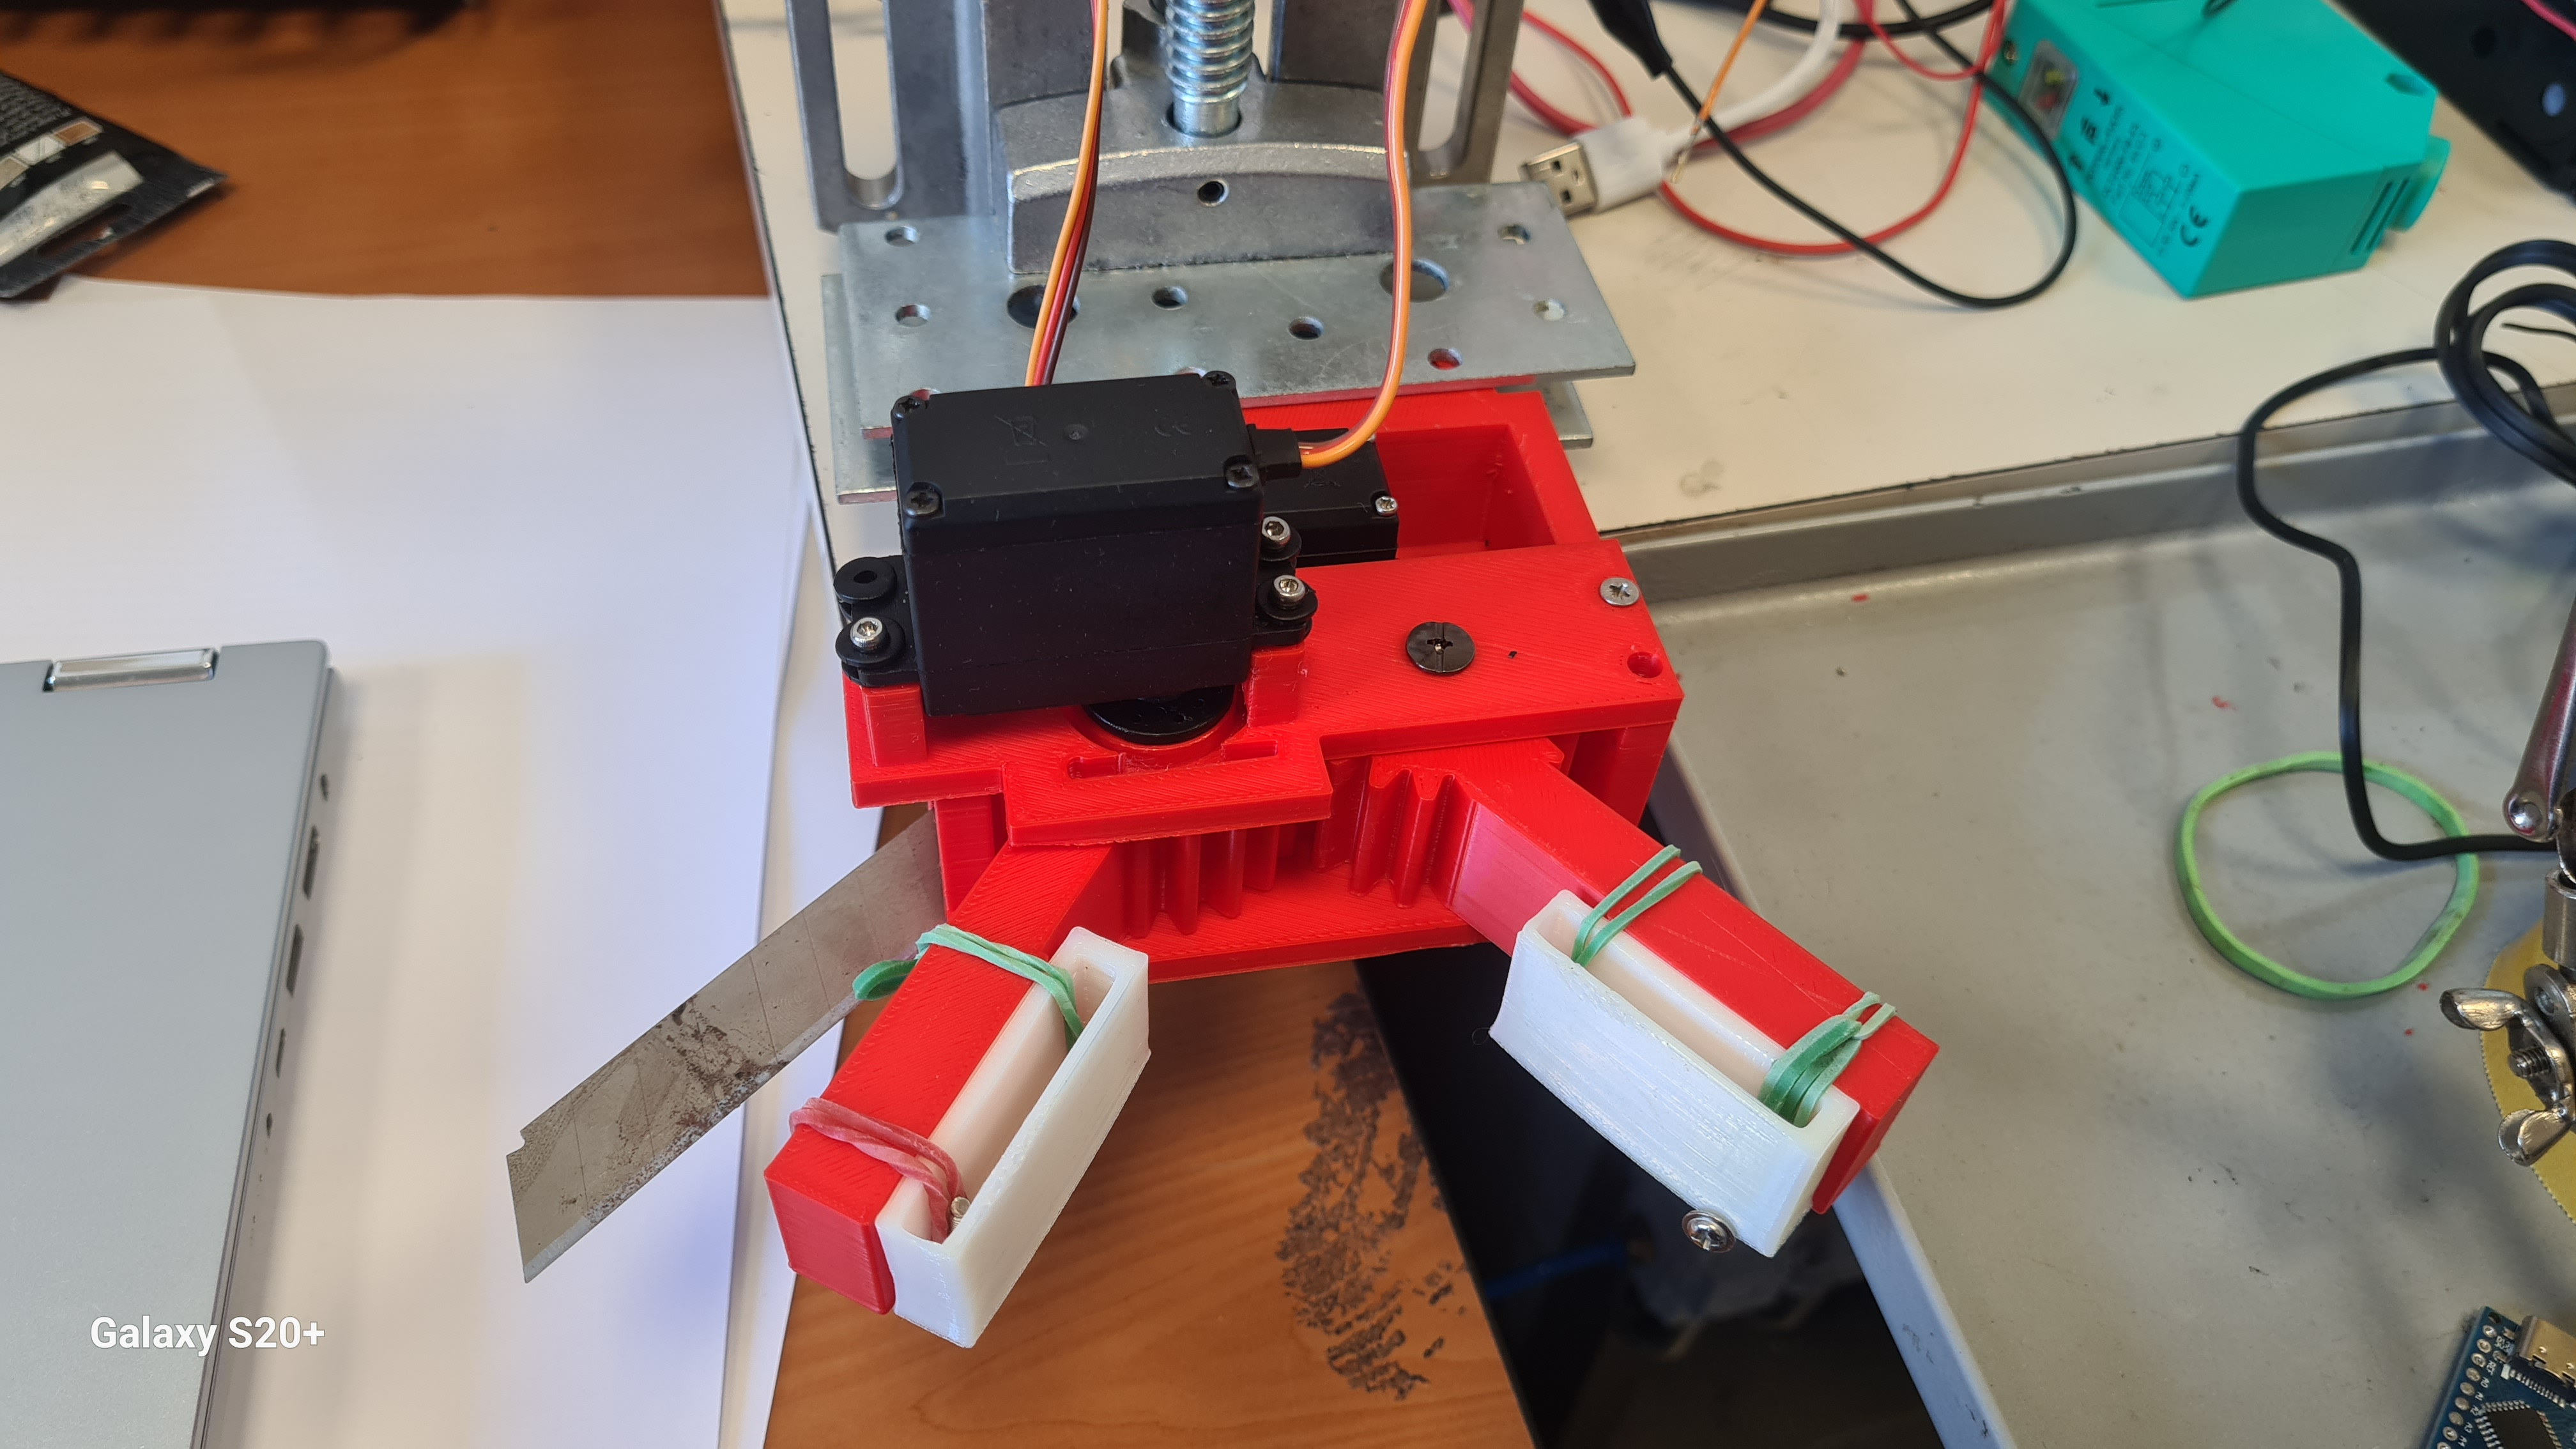
\includegraphics[width=0.85\textwidth]{Fingerfinal_design.jpg}
\caption{Assembled finger and blade module prototype.}
\label{fig:finger_final}
\end{figure}

Figure~\ref{fig:finger_final} shows the final assembly of the finger and blade module. The finger
pair is synchronised via the internal gear train and fitted with compliant pads to distribute
contact pressure, while the blade subassembly is mounted on a rigid bracket driven by a
high-torque servo.The material used for the pad is flexible filament which bends inwards under the pressure and thus does not damage the asparagus stem.The mechanical packaging preserves a compact envelope around the tool
centre point, ensuring that the cutting stroke clears the finger workspace and that cable
routing remains unobstructed. Assembly choices emphasised maintainability: the blade is
readily replaceable, servos are accessible for calibration, and all critical joints are supported by
bushings or bearings to limit wear. The design provides smooth, symmetric closing,
repeatable centring of the spear, and consistent cut quality across repeated cycles, indicating
that the prototype satisfies the principal design objectives for gentle, reliable harvesting.




